% Capítulo 4 — Análisis del Sistema (LocalMind-AI)
% Reescrito para el TFM; contenido original (no se reutiliza prosa del TFG).

Este capítulo presenta el análisis del sistema LocalMind-AI a partir de los requisitos identificados en el Capítulo~\ref{ch:requisitos}. El propósito es describir las interacciones entre la persona usuaria y el \gls{nanobot}, modeladas mediante casos de uso, diagramas de secuencia, de clases y de actividades siguiendo la especificación estándar de la Open Management Group \cite{omgUml2024} y la metodología de análisis orientado a objetos \cite{larmanIterativeIncrementalDevelopments2003}. El análisis se articula en torno a un único actor, la persona usuaria, que accede al sistema principalmente a través de una interfaz web desarrollada en Expo y React Native Web conectada mediante \gls{websocket}, contando con la \gls{tui} en Python y Rich para tareas de instalación, configuración y diagnóstico en entorno local.

El sistema LocalMind-AI es un asistente de \gls{ia} orientado a la ejecución local que combina razonamiento \gls{cot} con recuperación aumentada por generación mediante el protocolo \gls{cotrag}, apoyándose en herramientas externas a través del protocolo \gls{mcp}. Los motores de inferencia (\gls{ollama} y \gls{omlx}) y la base de conocimiento vectorial (\gls{chromadb}) operan íntegramente en el equipo de la persona usuaria, garantizando la privacidad de los datos descrita en el requisito no funcional RNF1.

\section{Diagrama de casos de uso}

La Figura~\ref{fig:diagramaCU} recoge los nueve casos de uso que cubren la totalidad de los requisitos funcionales (RF1 a RF10) y no funcionales (RNF1 a RNF14) definidos en el Capítulo~\ref{ch:requisitos}. El actor único es la persona usuaria, que interactúa con el sistema a través de la interfaz web o la \gls{tui}, conectadas mediante \gls{websocket} al puerto 8765 o mediante la API REST en el puerto 8900 del \gls{nanobot}.

\begin{figure}[h!tp]
  \centering
  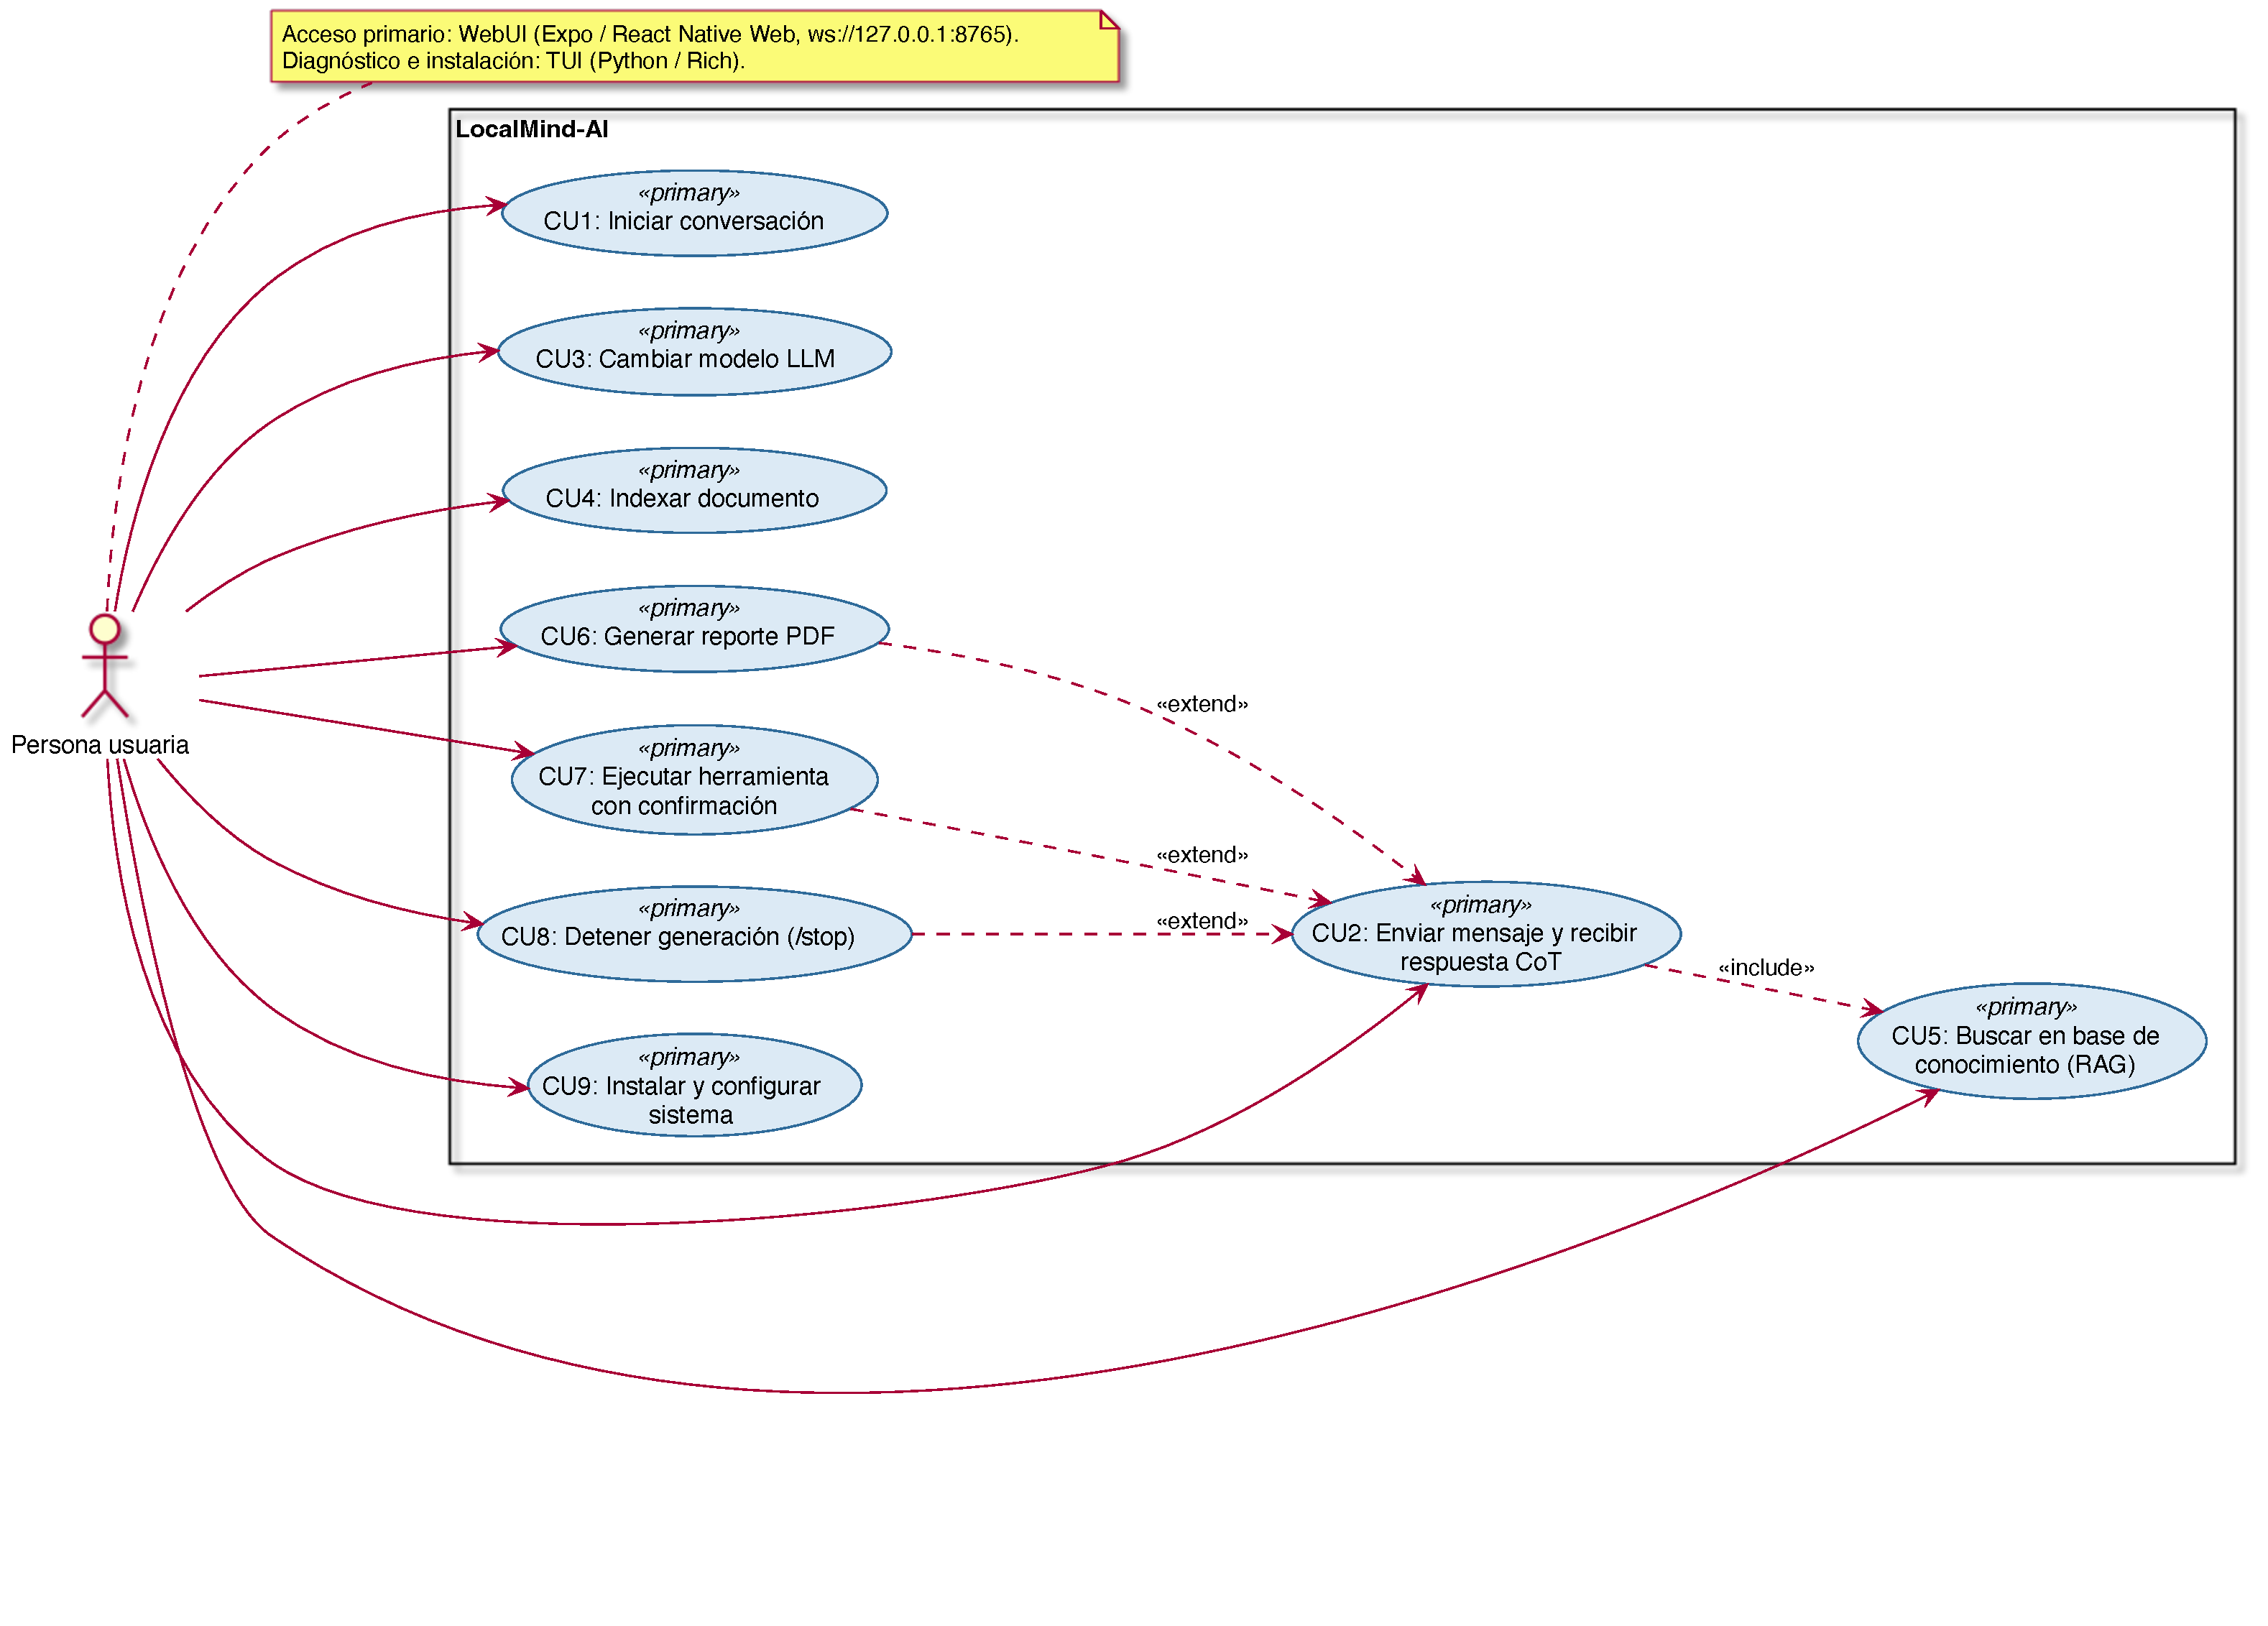
\includegraphics[width=0.9\textwidth]{figs/diagrama-casos-uso.pdf}
  \caption{Diagrama de casos de uso de LocalMind-AI.}
  \label{fig:diagramaCU}
\end{figure}

A continuación se detallan los nueve casos de uso del sistema. Cada tabla presenta las ocho secciones descriptivas estandarizadas \cite{omgUml2024} con el identificador, nombre, actores, descripción, flujo de datos principal, precondiciones, postcondiciones y requisitos asociados.

% Caso de Uso 1.
\begin{table}[h!tp]
  \centering
  \begin{adjustbox}{max width=\textwidth}
    \begin{tabular}{|>{\centering\arraybackslash}p{3cm}|p{8.5cm}|}
      \hline
      \textbf{Caso de Uso}      & CU1 \\ \hline
      \textbf{Nombre}           & Iniciar conversación \\ \hline
      \textbf{Actores}          & Persona usuaria (a través de WebUI o TUI) \\ \hline
      \textbf{Descripción}      & Establece una sesión conversacional con el sistema. El cliente abre un canal de comunicación con el \gls{nanobot} y crea un contexto de sesión persistente con identificador único. \\ \hline
      \textbf{Flujo de datos}   &
      \begin{minipage}[t]{\linewidth}
        \vspace{0.4em}
        \begin{enumerate}[leftmargin=*,noitemsep,topsep=2pt]
          \item La persona usuaria abre la aplicación cliente en la WebUI o en la TUI.
          \item El cliente establece la conexión \gls{websocket} al puerto 8765 o realiza una petición a la API REST.
          \item El componente \texttt{WebSocketChannel} acepta la conexión y notifica al gestor de canales.
          \item El componente \texttt{AgentLoop} genera una nueva sesión con su identificador único.
          \item Se inicializa el archivo de sesión \gls{jsonl} en el volumen de almacenamiento persistente.
          \item El cliente recibe la confirmación de sesión activa y lista para recibir entradas.
        \end{enumerate}
        \vspace{0.4em}
      \end{minipage} \\ \hline
      \textbf{Precondiciones}   & Los servicios del contenedor están en ejecución y el motor de inferencia local es accesible. \\ \hline
      \textbf{Postcondiciones}  & Sesión creada con identificador único, historial \gls{jsonl} inicializado y canal en estado activo. \\ \hline
      \textbf{Requisitos}       & RF1, RF2, RF8, RNF1, RNF4, RNF7 \\ \hline
    \end{tabular}
  \end{adjustbox}
  \caption{CU1. Iniciar conversación.}
  \label{tab:CU1}
\end{table}

% Caso de Uso 2.
\begin{table}[h!tp]
  \centering
  \begin{adjustbox}{max width=\textwidth}
    \begin{tabular}{|>{\centering\arraybackslash}p{3cm}|p{8.5cm}|}
      \hline
      \textbf{Caso de Uso}      & CU2 \\ \hline
      \textbf{Nombre}           & Enviar mensaje y recibir respuesta en streaming CoT \\ \hline
      \textbf{Actores}          & Persona usuaria (a través de WebUI o TUI) \\ \hline
      \textbf{Descripción}      & La persona usuaria envía un mensaje de texto y recibe la respuesta del \gls{llm} en fragmentos incrementales mediante emisión continua, con visibilidad de los pasos intermedios del razonamiento \gls{cotrag}. \\ \hline
      \textbf{Flujo de datos}   &
      \begin{minipage}[t]{\linewidth}
        \vspace{0.4em}
        \begin{enumerate}[leftmargin=*,noitemsep,topsep=2pt]
          \item La persona usuaria escribe y envía un mensaje de texto.
          \item El cliente transmite el mensaje \texttt{new\_chat} a través del canal \gls{websocket}.
          \item El componente \texttt{WebSocketChannel} recibe el mensaje y lo publica en la barra de eventos.
          \item El método de procesamiento del agente invoca al constructor de contexto para enriquecer la solicitud con el historial, la memoria y los documentos recuperados.
          \item El ejecutor del agente invoca al proveedor del modelo con el contexto construido.
          \item El proveedor consulta al motor de inferencia seleccionado.
          \item El motor genera tokens de forma incremental.
          \item Cada token se envía como un paquete incremental al cliente mediante \gls{websocket}.
          \item Al recibir el token de finalización, se emite el evento de cierre y se guarda la respuesta en el archivo de sesión.
        \end{enumerate}
        \vspace{0.4em}
      \end{minipage} \\ \hline
      \textbf{Precondiciones}   & Sesión activa iniciada previamente en el caso de uso CU1 y canal de comunicación operativo. \\ \hline
      \textbf{Postcondiciones}  & Respuesta completa almacenada en el historial y renderizada correctamente en el cliente. \\ \hline
      \textbf{Requisitos}       & RF1, RF2, RF10, RNF2, RNF3, RNF7 \\ \hline
    \end{tabular}
  \end{adjustbox}
  \caption{CU2. Enviar mensaje y recibir respuesta en streaming CoT.}
  \label{tab:CU2}
\end{table}

% Caso de Uso 3.
\begin{table}[h!tp]
  \centering
  \begin{adjustbox}{max width=\textwidth}
    \begin{tabular}{|>{\centering\arraybackslash}p{3cm}|p{8.5cm}|}
      \hline
      \textbf{Caso de Uso}      & CU3 \\ \hline
      \textbf{Nombre}           & Cambiar modelo LLM \\ \hline
      \textbf{Actores}          & Persona usuaria (a través de WebUI o TUI) \\ \hline
      \textbf{Descripción}      & La persona usuaria alterna dinámicamente entre \gls{ollama} y \gls{omlx} como motor de inferencia activo, o cambia la variante del modelo sin necesidad de reiniciar la sesión. \\ \hline
      \textbf{Flujo de datos}   &
      \begin{minipage}[t]{\linewidth}
        \vspace{0.4em}
        \begin{enumerate}[leftmargin=*,noitemsep,topsep=2pt]
          \item La persona usuaria accede al panel de selección de modelos en la interfaz.
          \item Selecciona el motor de inferencia objetivo y la variante de cuantización deseada.
          \item El cliente envía la solicitud de cambio de proveedor al agente.
          \item El bucle del agente actualiza la instancia del proveedor de \gls{llm} con el nuevo motor.
          \item Se realiza una prueba de conectividad con el nuevo proveedor.
          \item Se notifica la confirmación del cambio al cliente.
        \end{enumerate}
        \vspace{0.4em}
      \end{minipage} \\ \hline
      \textbf{Precondiciones}   & Al menos un motor de inferencia local en ejecución y accesible durante una sesión activa. \\ \hline
      \textbf{Postcondiciones}  & Proveedor reconfigurado para que las siguientes peticiones empleen el nuevo motor seleccionado. \\ \hline
      \textbf{Requisitos}       & RF3, RNF4, RNF9 \\ \hline
    \end{tabular}
  \end{adjustbox}
  \caption{CU3. Cambiar modelo \gls{llm}.}
  \label{tab:CU3}
\end{table}

% Caso de Uso 4.
\begin{table}[h!tp]
  \centering
  \begin{adjustbox}{max width=\textwidth}
    \begin{tabular}{|>{\centering\arraybackslash}p{3cm}|p{8.5cm}|}
      \hline
      \textbf{Caso de Uso}      & CU4 \\ \hline
      \textbf{Nombre}           & Indexar documento en base de conocimiento \\ \hline
      \textbf{Actores}          & Persona usuaria (a través de WebUI) \\ \hline
      \textbf{Descripción}      & La persona usuaria sube un archivo en formato \gls{pdf} o \gls{markdown} que se procesa, se trocea en fragmentos semánticos y se indexa como vectores en \gls{chromadb}. \\ \hline
      \textbf{Flujo de datos}   &
      \begin{minipage}[t]{\linewidth}
        \vspace{0.4em}
        \begin{enumerate}[leftmargin=*,noitemsep,topsep=2pt]
          \item La persona usuaria selecciona un documento en formato \gls{pdf} o \gls{markdown}.
          \item El cliente envía el archivo al servicio a través del punto de entrada de carga.
          \item El agente extrae el contenido textual del archivo recibido.
          \item Se fragmenta el texto mediante división recursiva con solapamiento semántico.
          \item La función de vectorización genera los vectores correspondientes utilizando el servicio local.
          \item Los fragmentos y sus vectores se insertan en la colección de \gls{chromadb}.
          \item Se notifica la finalización indicando el recuento de fragmentos indexados.
        \end{enumerate}
        \vspace{0.4em}
      \end{minipage} \\ \hline
      \textbf{Precondiciones}   & Base de datos vectorial \gls{chromadb} accesible y servicio local de vectorización activo. \\ \hline
      \textbf{Postcondiciones}  & Documento fragmentado e indexado en la base vectorial para consultas futuras. \\ \hline
      \textbf{Requisitos}       & RF4, RF5, RNF5, RNF12 \\ \hline
    \end{tabular}
  \end{adjustbox}
  \caption{CU4. Indexar documento en base de conocimiento.}
  \label{tab:CU4}
\end{table}

% Caso de Uso 5.
\begin{table}[h!tp]
  \centering
  \begin{adjustbox}{max width=\textwidth}
    \begin{tabular}{|>{\centering\arraybackslash}p{3cm}|p{8.5cm}|}
      \hline
      \textbf{Caso de Uso}      & CU5 \\ \hline
      \textbf{Nombre}           & Buscar en base de conocimiento (RAG) \\ \hline
      \textbf{Actores}          & Persona usuaria (a través de WebUI) o invocado por CU2 \\ \hline
      \textbf{Descripción}      & Transforma la consulta en un vector, recupera los fragmentos más afines de la base vectorial \gls{chromadb} e inyecta dicho contexto en la solicitud al \gls{llm}. \\ \hline
      \textbf{Flujo de datos}   &
      \begin{minipage}[t]{\linewidth}
        \vspace{0.4em}
        \begin{enumerate}[leftmargin=*,noitemsep,topsep=2pt]
          \item Se recibe una consulta directa o procedente del flujo \gls{cotrag} en el caso de uso CU2.
          \item El constructor de contexto convierte la consulta en vector mediante la función de vectorización local.
          \item Se consulta la colección de \gls{chromadb} extrayendo los fragmentos más próximos.
          \item Se aplican los filtros correspondientes por umbral de similitud semántica.
          \item Los fragmentos seleccionados se inyectan en el contexto de la solicitud.
          \item El modelo genera la respuesta fundamentada en la información recuperada.
        \end{enumerate}
        \vspace{0.4em}
      \end{minipage} \\ \hline
      \textbf{Precondiciones}   & Al menos un documento indexado en \gls{chromadb} y servicio de vectorización disponible. \\ \hline
      \textbf{Postcondiciones}  & Contexto relevante inyectado en la sesión para la generación de la respuesta. \\ \hline
      \textbf{Requisitos}       & RF5, RNF6, RNF12, RNF14 \\ \hline
    \end{tabular}
  \end{adjustbox}
  \caption{CU5. Buscar en base de conocimiento (\gls{rag}).}
  \label{tab:CU5}
\end{table}

% Caso de Uso 6.
\begin{table}[h!tp]
  \centering
  \begin{adjustbox}{max width=\textwidth}
    \begin{tabular}{|>{\centering\arraybackslash}p{3cm}|p{8.5cm}|}
      \hline
      \textbf{Caso de Uso}      & CU6 \\ \hline
      \textbf{Nombre}           & Generar reporte PDF \\ \hline
      \textbf{Actores}          & Persona usuaria (a través del agente) \\ \hline
      \textbf{Descripción}      & El agente ejecuta la herramienta \gls{mcp} encargada de generar informes para confeccionar un documento en formato \gls{pdf} a partir del contenido de la sesión. \\ \hline
      \textbf{Flujo de datos}   &
      \begin{minipage}[t]{\linewidth}
        \vspace{0.4em}
        \begin{enumerate}[leftmargin=*,noitemsep,topsep=2pt]
          \item El \gls{llm} determina la necesidad de generar un documento y emite una llamada a herramienta.
          \item El ejecutor del agente captura la llamada y consulta el registro de herramientas.
          \item El registro redirige la petición al servidor de herramientas \gls{mcp}.
          \item El servidor ejecuta la función de generación mediante un subproceso conectado por entrada y salida estándar.
          \item El archivo en formato \gls{pdf} se guarda en el espacio de trabajo local persistente.
          \item Se devuelve la confirmación y la ruta del archivo al agente para informar a la persona usuaria.
        \end{enumerate}
        \vspace{0.4em}
      \end{minipage} \\ \hline
      \textbf{Precondiciones}   & Servidor de herramientas \gls{mcp} activo y herramienta registrada correctamente. \\ \hline
      \textbf{Postcondiciones}  & Documento en formato \gls{pdf} creado y almacenado localmente en el directorio de trabajo. \\ \hline
      \textbf{Requisitos}       & RF9, RF10, RNF6, RNF11 \\ \hline
    \end{tabular}
  \end{adjustbox}
  \caption{CU6. Generar reporte \gls{pdf}.}
  \label{tab:CU6}
\end{table}

% Caso de Uso 7.
\begin{table}[h!tp]
  \centering
  \begin{adjustbox}{max width=\textwidth}
    \begin{tabular}{|>{\centering\arraybackslash}p{3cm}|p{8.5cm}|}
      \hline
      \textbf{Caso de Uso}      & CU7 \\ \hline
      \textbf{Nombre}           & Ejecutar herramienta con confirmación \\ \hline
      \textbf{Actores}          & Persona usuaria (a través de WebUI o TUI) \\ \hline
      \textbf{Descripción}      & El agente solicita ejecutar una acción sensible o protegida mediante \gls{mcp}, requiriendo la autorización explícita de la persona usuaria antes de su ejecución. \\ \hline
      \textbf{Flujo de datos}   &
      \begin{minipage}[t]{\linewidth}
        \vspace{0.4em}
        \begin{enumerate}[leftmargin=*,noitemsep,topsep=2pt]
          \item El modelo emite una orden de ejecución de herramienta clasificada como protegida.
          \item El ejecutor del agente detecta la política de confirmación e interrumpe el flujo.
          \item El cliente muestra un diálogo emergente de confirmación con las opciones de aceptar, rechazar o autorizar siempre en lista blanca.
          \item La persona usuaria selecciona una opción en la interfaz.
          \item En caso de aceptación, la herramienta se ejecuta y se retorna el resultado al agente.
          \item En caso de rechazo, la ejecución se cancela y se notifica la decisión al modelo.
        \end{enumerate}
        \vspace{0.4em}
      \end{minipage} \\ \hline
      \textbf{Precondiciones}   & Solicitud de herramienta protegida emitida por el agente y cliente conectado. \\ \hline
      \textbf{Postcondiciones}  & Acción autorizada y ejecutada o bien rechazada y abortada de forma segura. \\ \hline
      \textbf{Requisitos}       & RF9, RF10, RNF6 \\ \hline
    \end{tabular}
  \end{adjustbox}
  \caption{CU7. Ejecutar herramienta con confirmación.}
  \label{tab:CU7}
\end{table}

% Caso de Uso 8.
\begin{table}[h!tp]
  \centering
  \begin{adjustbox}{max width=\textwidth}
    \begin{tabular}{|>{\centering\arraybackslash}p{3cm}|p{8.5cm}|}
      \hline
      \textbf{Caso de Uso}      & CU8 \\ \hline
      \textbf{Nombre}           & Detener generación (\texttt{/stop}) \\ \hline
      \textbf{Actores}          & Persona usuaria (a través de WebUI o TUI) \\ \hline
      \textbf{Descripción}      & La persona usuaria cancela de inmediato la generación de tokens en curso, manteniendo la sesión conversacional activa y guardando el contenido parcial. \\ \hline
      \textbf{Flujo de datos}   &
      \begin{minipage}[t]{\linewidth}
        \vspace{0.4em}
        \begin{enumerate}[leftmargin=*,noitemsep,topsep=2pt]
          \item La persona usuaria presiona el botón de cancelación o envía la orden \texttt{/stop}.
          \item El cliente envía la señal de interrupción mediante el canal \gls{websocket}.
          \item El bucle del agente interrumpe el proceso en curso y cancela la petición al motor de inferencia.
          \item El proveedor del modelo cierra la conexión de emisión continua.
          \item Se envía el evento de cierre con estado cancelado.
          \item La respuesta parcial generada hasta el momento se guarda en el historial de sesión.
        \end{enumerate}
        \vspace{0.4em}
      \end{minipage} \\ \hline
      \textbf{Precondiciones}   & Generación activa en curso en el canal de comunicación. \\ \hline
      \textbf{Postcondiciones}  & Generación interrumpida, canal de comunicación en estado de espera e historial actualizado. \\ \hline
      \textbf{Requisitos}       & RF2, RF10, RNF7, RNF10 \\ \hline
    \end{tabular}
  \end{adjustbox}
  \caption{CU8. Detener generación (\texttt{/stop}).}
  \label{tab:CU8}
\end{table}

% Caso de Uso 9.
\begin{table}[h!tp]
  \centering
  \begin{adjustbox}{max width=\textwidth}
    \begin{tabular}{|>{\centering\arraybackslash}p{3cm}|p{8.5cm}|}
      \hline
      \textbf{Caso de Uso}      & CU9 \\ \hline
      \textbf{Nombre}           & Instalar y configurar sistema \\ \hline
      \textbf{Actores}          & Persona usuaria (a través de TUI) \\ \hline
      \textbf{Descripción}      & La persona usuaria ejecuta la \gls{tui} para automatizar la comprobación de requisitos, la generación del archivo de entorno, el despliegue de contenedores y la descarga de modelos. \\ \hline
      \textbf{Flujo de datos}   &
      \begin{minipage}[t]{\linewidth}
        \vspace{0.4em}
        \begin{enumerate}[leftmargin=*,noitemsep,topsep=2pt]
          \item La persona usuaria inicia la \gls{tui} ejecutable o el script de inicio.
          \item La interfaz comprueba los requisitos del sistema como versión de Docker, arquitectura, memoria y disco.
          \item Se crea o actualiza el archivo de configuración de variables de entorno.
          \item Se ejecuta el despliegue mediante Docker Compose iniciando los servicios correspondientes.
          \item Se descargan los modelos de inferencia seleccionados si no están almacenados en caché.
          \item Se realizan comprobaciones de estado de salud en todos los servicios.
          \item La \gls{tui} notifica que el sistema está completamente operativo.
        \end{enumerate}
        \vspace{0.4em}
      \end{minipage} \\ \hline
      \textbf{Precondiciones}   & Permisos de ejecución y entorno Docker instalado en el equipo del usuario. \\ \hline
      \textbf{Postcondiciones}  & Servicios e infraestructura Docker operativos con los modelos descargados y validados. \\ \hline
      \textbf{Requisitos}       & RF10, RNF4, RNF10, RNF11 \\ \hline
    \end{tabular}
  \end{adjustbox}
  \caption{CU9. Instalar y configurar sistema.}
  \label{tab:CU9}
\end{table}

\FloatBarrier

\section{Diagrama general de secuencia del sistema}

La Figura~\ref{fig:diagramaSG} presenta el diagrama de secuencia que describe el flujo completo de una interacción conversacional con LocalMind-AI, desde el envío del mensaje hasta la recepción de la respuesta en formato continuo, incluyendo las ramas de invocación de herramientas, confirmación de acciones protegidas y gestión de errores.

\begin{figure}[h!tp]
  \centering
  \includegraphics[width=1.0\textwidth]{figs/diagrama-secuencia-general.pdf}
  \caption{Diagrama general de secuencia del sistema.}
  \label{fig:diagramaSG}
\end{figure}

El flujo principal se inicia cuando la persona usuaria envía un mensaje desde la WebUI desarrollada en Expo y React Native Web. El cliente encapsula el mensaje en una estructura \texttt{new\_chat} y la transmite al componente \texttt{WebSocketChannel} a través del \gls{websocket} en el puerto 8765. El canal publica el mensaje en la barra de eventos \texttt{MessageBus}, que lo entrega al bucle principal del agente \texttt{AgentLoop}. Este componente coordina el proceso invocando en primer lugar al constructor de contexto \texttt{ContextBuilder} para compilar el historial de sesión, la memoria engram y los fragmentos relevantes recuperados de \gls{chromadb} según el protocolo \gls{cotrag}. A continuación, delega en el ejecutor \texttt{AgentRunner} la realización del bucle de razonamiento.

El ejecutor \texttt{AgentRunner} invoca al proveedor de lenguaje \texttt{LLMProvider}, representado concretamente por la clase \texttt{OpenAICompatProvider}, la cual actúa como adaptador tanto para \gls{ollama} en el puerto 11434 como para \gls{omlx} en el puerto 8082 accesibles en el entorno local. El motor de inferencia genera tokens de forma incremental que se transmiten al cliente como paquetes de emisión continua a través de la cadena formada por el ejecutor, el bucle del agente, la barra de eventos, el canal de comunicación y la interfaz de usuario. El flujo concluye cuando se recibe el token de finalización, momento en el cual la respuesta completa se guarda en el historial \gls{jsonl}.

Cuando el modelo decide invocar una herramienta externa, el ejecutor del agente consulta el registro de herramientas \texttt{ToolRegistry} para localizar el servidor \texttt{McpToolsServer} correspondiente y le envía los parámetros a través del protocolo \gls{mcp} en un subproceso por entrada y salida estándar. Si la herramienta está clasificada como protegida por la política de seguridad, el sistema solicita confirmación a la persona usuaria antes de ejecutarla, ofreciendo las alternativas de aceptar, rechazar o autorizar siempre. En caso de rechazo, la ejecución se cancela y se notifica la interrupción al agente.

El diagrama contempla asimismo dos escenarios de error. Si el motor de inferencia no responde por superar el tiempo de espera de diez segundos o por inaccesibilidad del servicio, el bucle del agente genera un mensaje de error comprensible y lo transmite al cliente ofreciendo la posibilidad de reintentar la operación. Por otra parte, si la base vectorial \gls{chromadb} no se encuentra disponible durante la fase de construcción de contexto, el sistema omite la etapa de recuperación e informa del incidente al módulo de observabilidad para continuar con la inferencia directa según el requisito RNF13.

\section{Diagrama de clases general}

La Figura~\ref{fig:diagramaCG} muestra el diagrama de clases que representa la estructura estática del sistema, organizada en tres paquetes principales denominados Agente, Proveedores y Canales y Cliente y Persistencia.

\begin{figure}[h!tp]
  \centering
  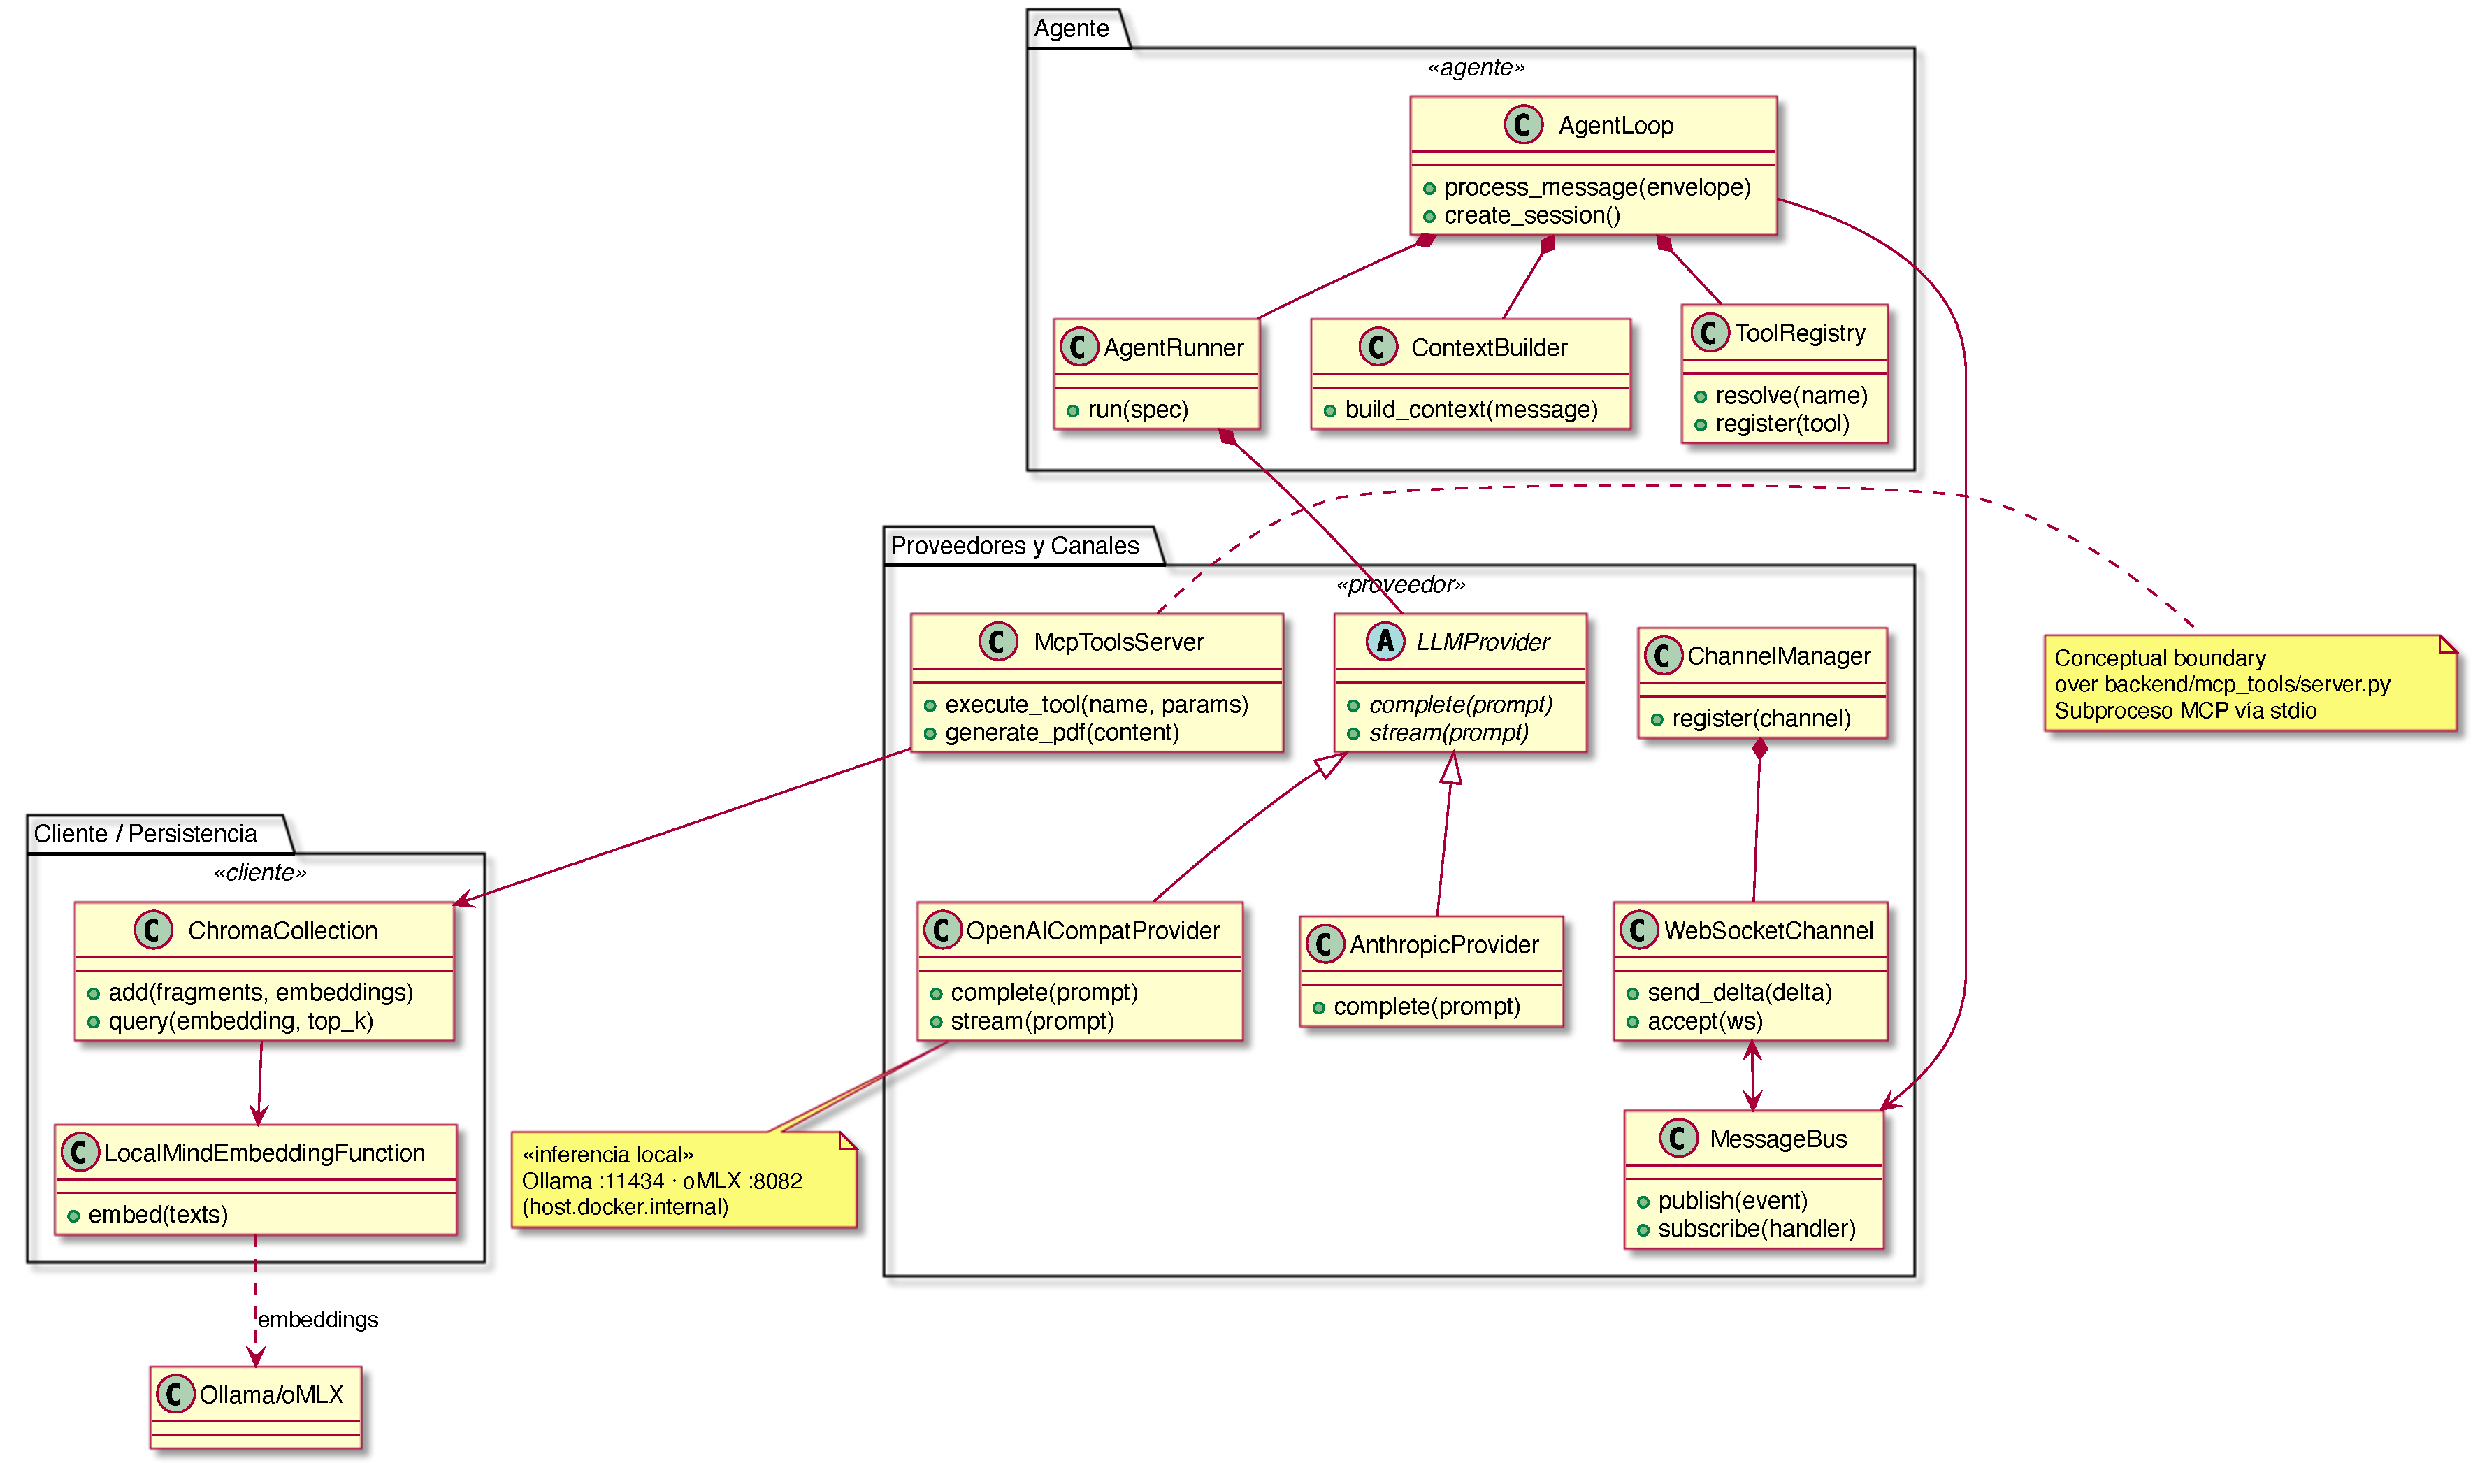
\includegraphics[width=1.0\textwidth]{figs/diagrama-clases-general.pdf}
  \caption{Diagrama de clases general del sistema.}
  \label{fig:diagramaCG}
\end{figure}

El paquete Agente agrupa las clases que implementan la lógica conversacional. La clase \texttt{AgentLoop} actúa como raíz del agregado y compone a \texttt{AgentRunner}, encargada del bucle de razonamiento y la coordinación de llamadas a herramientas, a \texttt{ContextBuilder}, responsable de ensamblar el contexto con el historial, la memoria y la información de la base vectorial, y a \texttt{ToolRegistry}, que mantiene el registro de herramientas \gls{mcp} disponibles. Las relaciones de composición se representan gráficamente mediante líneas con rombo negro relleno, indicando formalmente que el bucle del agente posee y administra el ciclo de vida de estos colaboradores principales.

El paquete Proveedores y Canales contiene las clases que gestionan la inferencia, los canales de comunicación y las herramientas externas. La clase abstracta \texttt{LLMProvider} define los métodos de generación completa y continua, siendo heredada por \texttt{OpenAICompatProvider} y \texttt{AnthropicProvider}. La clase \texttt{OpenAICompatProvider} constituye el adaptador de inferencia local para los motores \gls{ollama} en el puerto 11434 y \gls{omlx} en el puerto 8082. Por su parte, \texttt{ChannelManager} administra el canal activo \texttt{WebSocketChannel} en el puerto 8765. La barra de eventos \texttt{MessageBus} desacopla la recepción de mensajes del procesamiento del agente, mientras que \texttt{McpToolsServer} representa el servidor de herramientas \gls{mcp} que se ejecuta en subproceso con comunicación por entrada y salida estándar.

El paquete Cliente y Persistencia agrupa a \texttt{ChromaCollection}, que abstrae las colecciones de la base vectorial \gls{chromadb} para almacenar y consultar vectores, y a \texttt{LocalMindEmbeddingFunction}, que delega en el motor de inferencia local para generar los vectores correspondientes. La relación de dependencia entre ambas clases indica que la colección de \gls{chromadb} utiliza dicha función para convertir los textos en vectores antes de su almacenamiento o consulta.

\section{Diagramas de actividades más relevantes del análisis}

Esta sección presenta dos diagramas de actividades complementarios que describen los flujos operativos más densos y relevantes del sistema: el protocolo de razonamiento \gls{cotrag} del agente, en la Figura~\ref{fig:diagramaAP1}, y el flujo de comunicación y ciclo de vida del canal \gls{websocket}, en la Figura~\ref{fig:diagramaAP2}.

\subsection{Protocolo CoT-RAG}

La Figura~\ref{fig:diagramaAP1} describe el diagrama de actividades de cinco pasos que el agente sigue para procesar cada mensaje recibido de la persona usuaria.

\begin{figure}[h!tp]
  \centering
  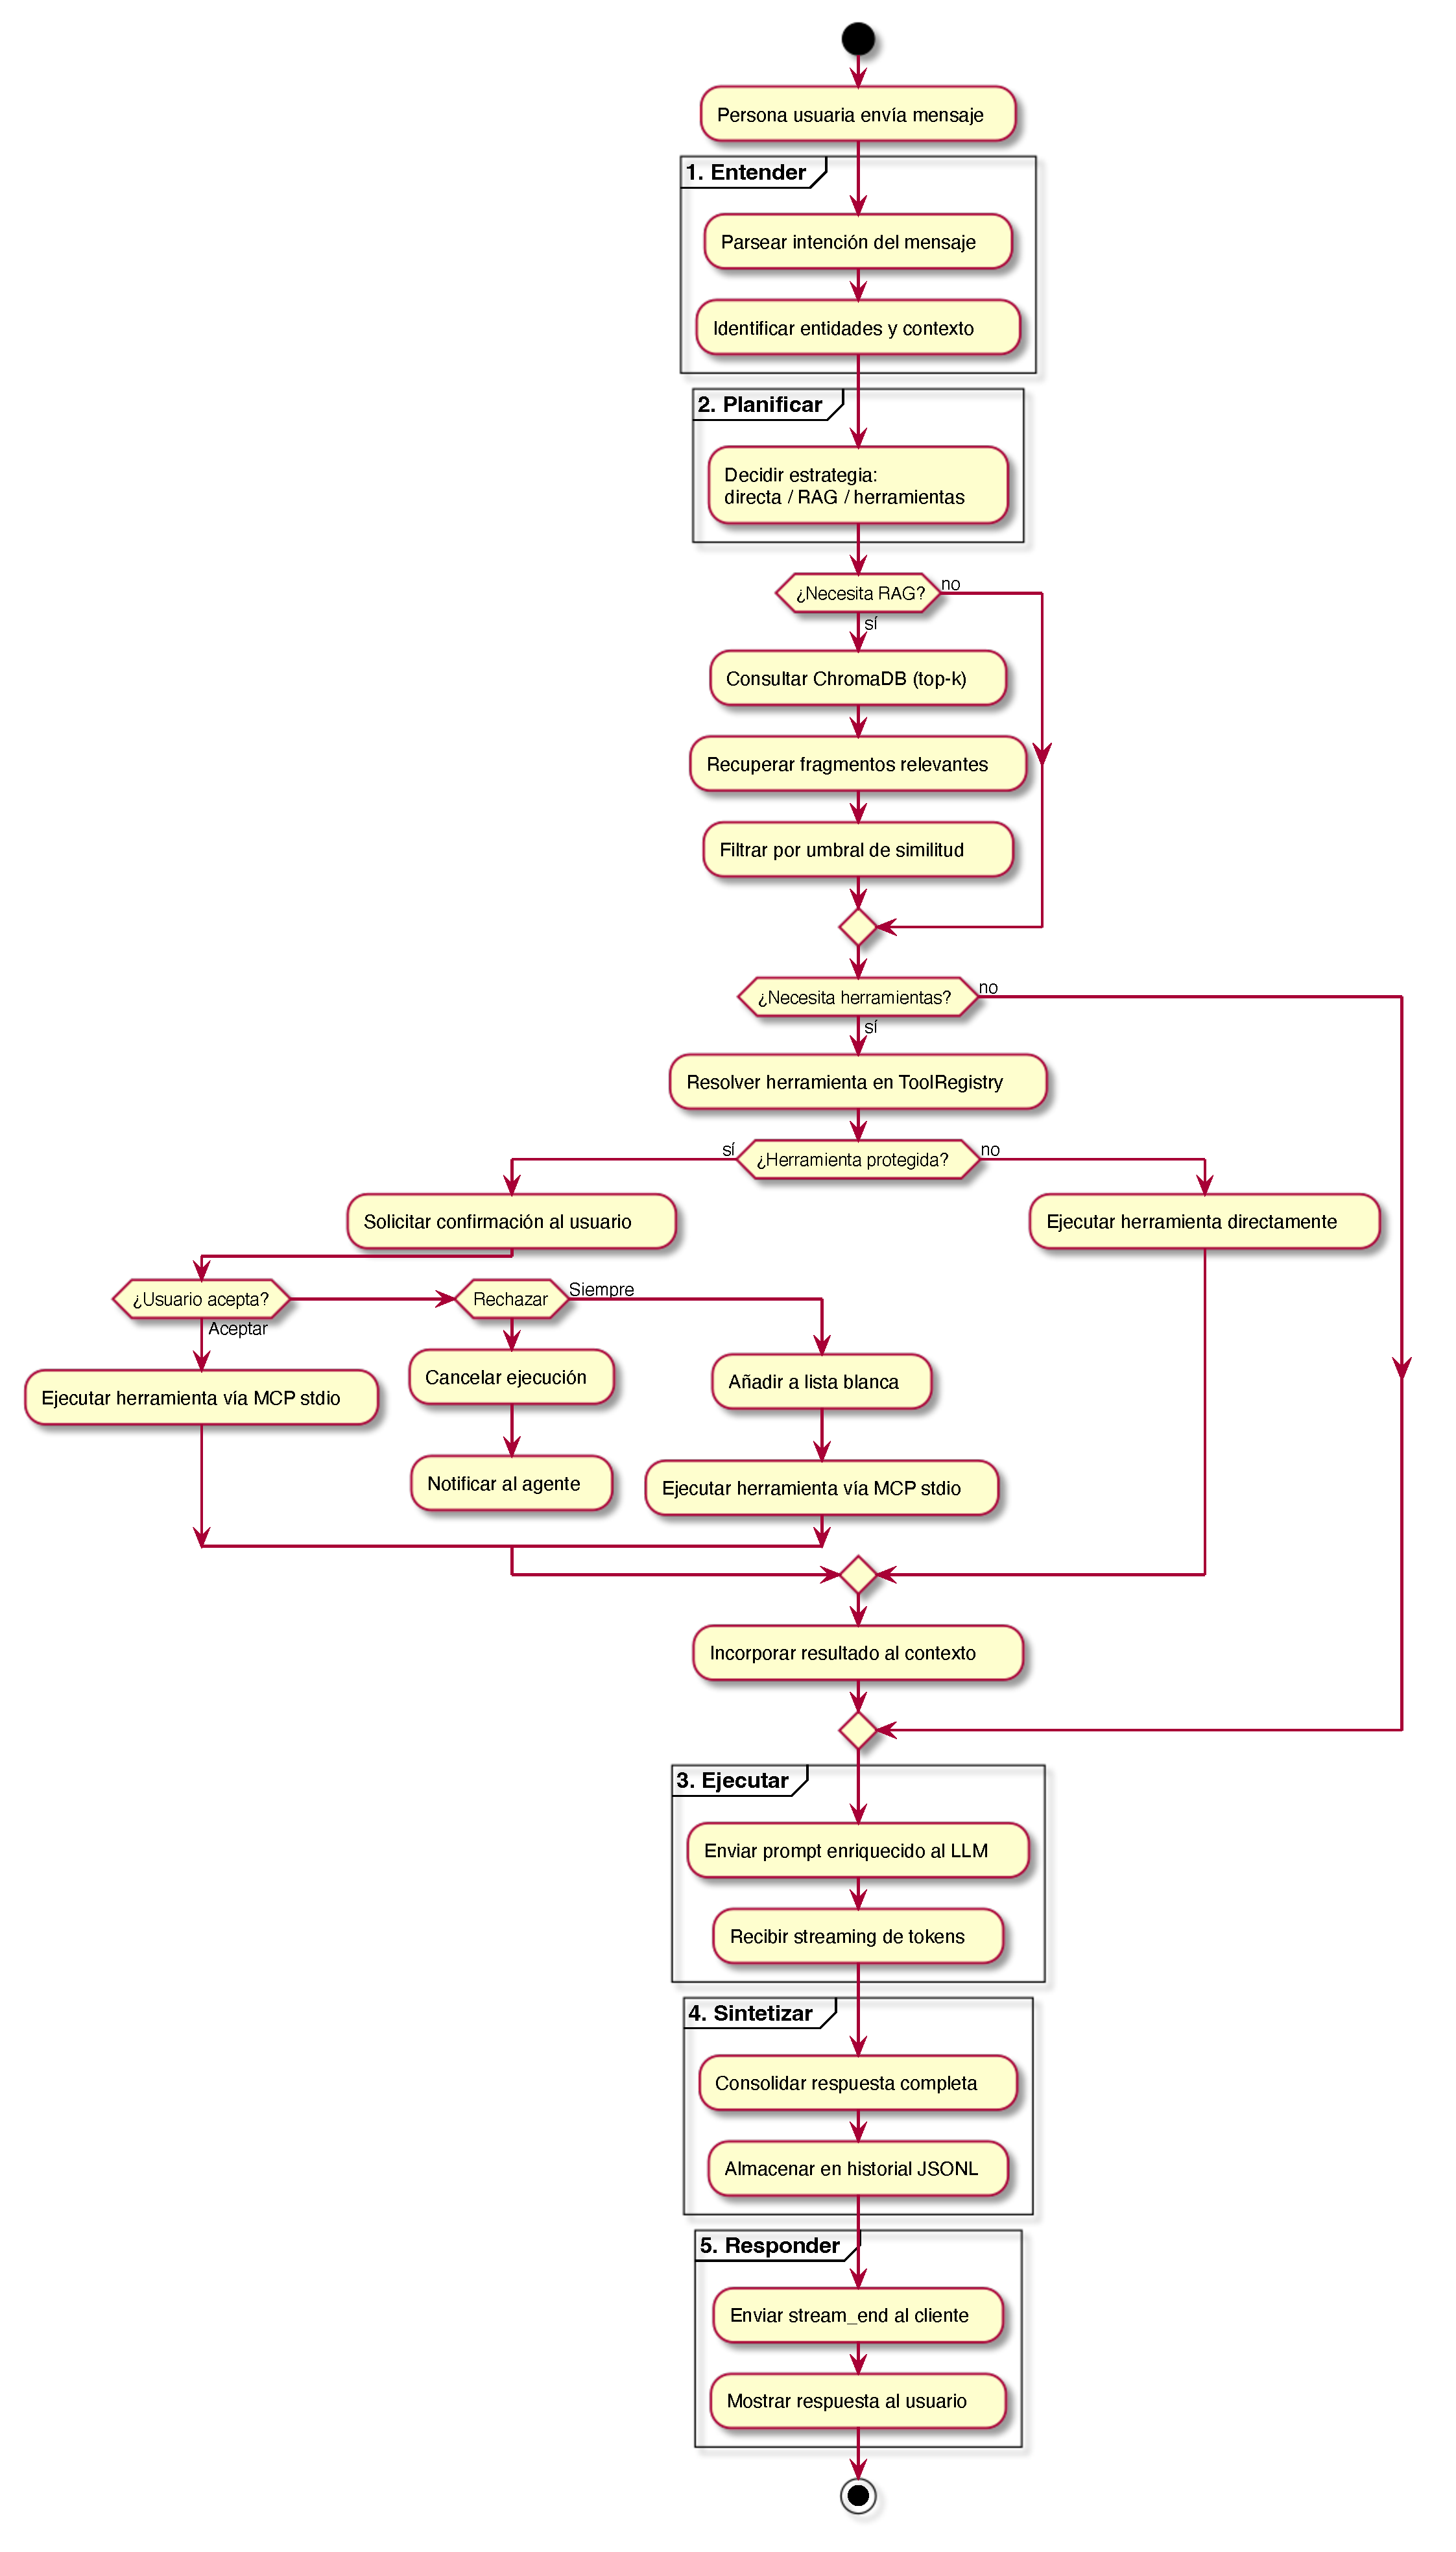
\includegraphics[width=\textwidth, height=0.82\textheight, keepaspectratio]{figs/diagrama-actividades-cot-rag.pdf}
  \caption{Diagrama de actividades del protocolo \gls{cotrag}.}
  \label{fig:diagramaAP1}
\end{figure}

El protocolo se inicia con la fase de comprensión, en la que el agente analiza la intención del mensaje e identifica las entidades y el contexto relevantes. A continuación, la fase de planificación decide la estrategia a seguir mediante respuesta directa, consulta a la base de conocimiento, invocación de herramientas o una combinación de las mismas.

Si el agente determina que requiere información de la base de conocimiento, se ejecuta la fase de búsqueda vectorial consultando \gls{chromadb} con los vectores de la solicitud, recuperando los fragmentos más próximos y filtrándolos por el umbral de similitud semántica establecido en el caso de uso CU5. Si la estrategia contempla invocar herramientas, el agente localiza la herramienta en el registro y la ejecuta mediante el servidor \gls{mcp}. Cuando la herramienta se encuentra clasificada como protegida, se solicita la confirmación explícita de la persona usuaria, quien puede aceptar, rechazar o autorizar la herramienta en lista blanca. En caso de rechazo, la ejecución se cancela y se notifica la interrupción al agente.

Tras la fase de ejecución, el agente pasa a la fase de síntesis, en la cual consolida la respuesta completa, integra los resultados de las herramientas y el contexto recuperado, y guarda la respuesta en el archivo de sesión. Finalmente, la fase de respuesta envía el evento de cierre al cliente y muestra el resultado en la interfaz.

\subsection{Ciclo de vida y comunicación del WebSocket}

La Figura~\ref{fig:diagramaAP2} detalla el diagrama de actividades que rige el establecimiento de la conexión \gls{websocket}, la recepción de eventos, la emisión en emisión continua y la gestión de reconexiones automáticas ante fallos de red.

\begin{figure}[h!tp]
  \centering
  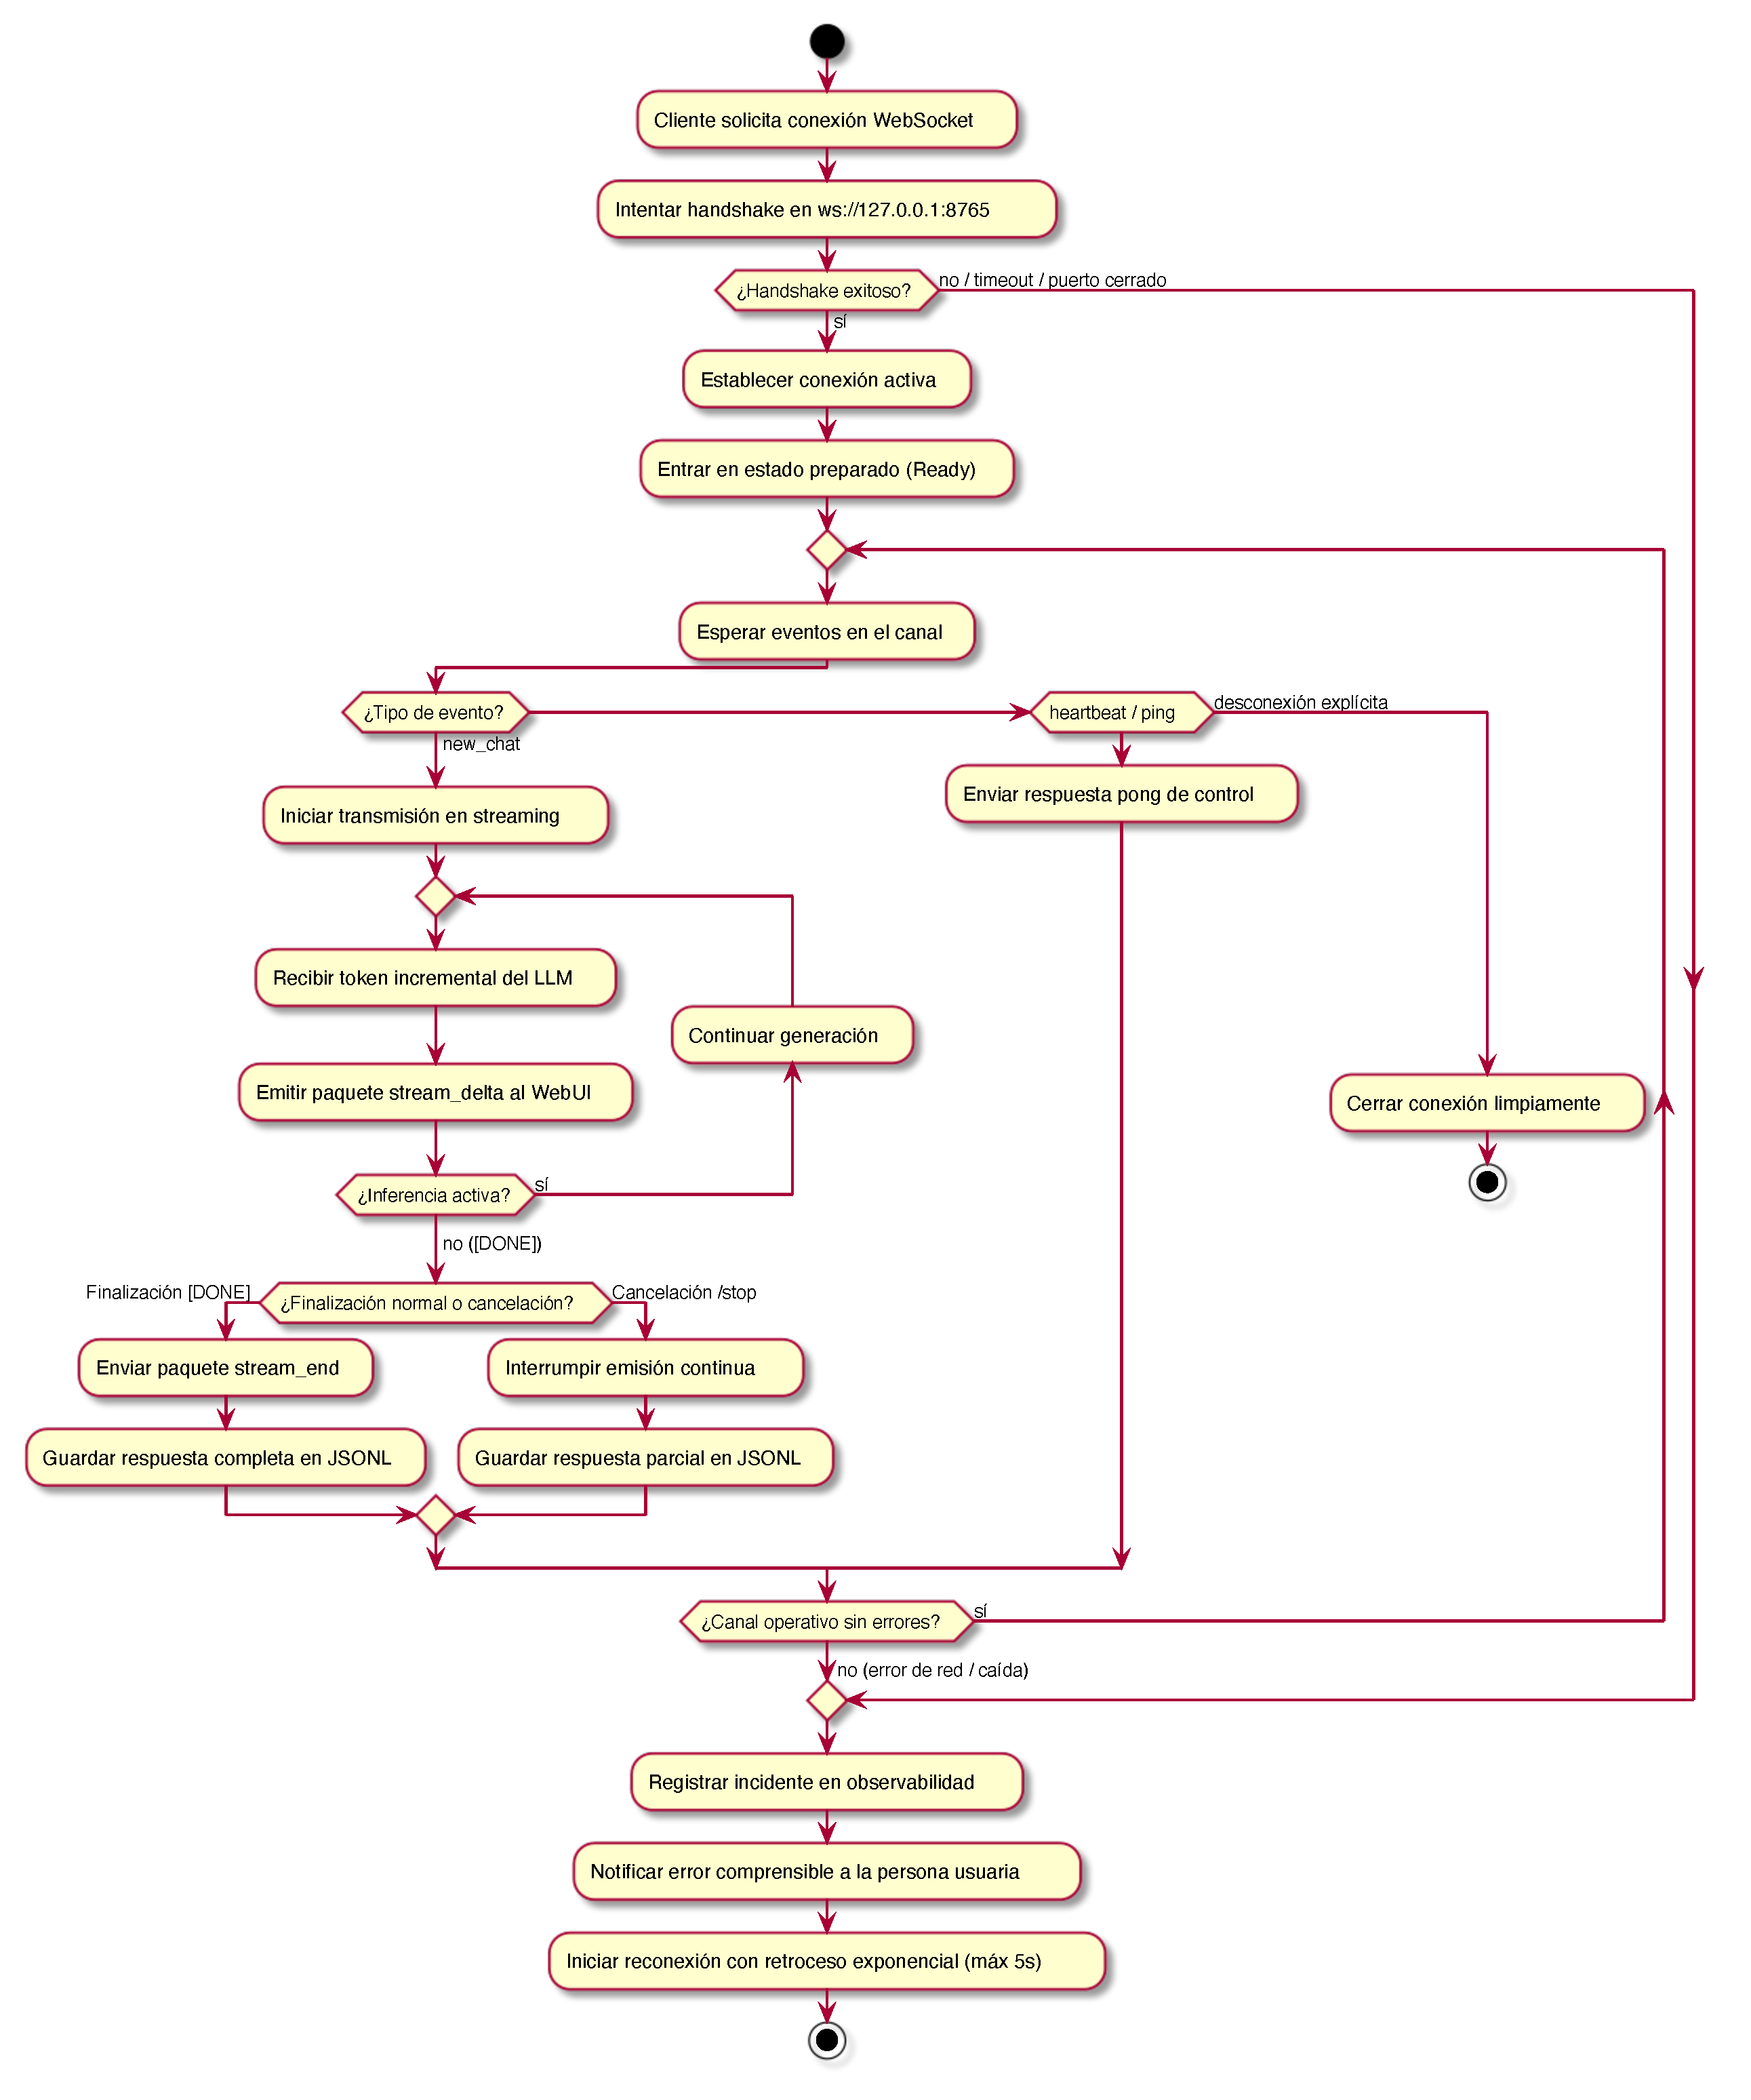
\includegraphics[width=\textwidth, height=0.82\textheight, keepaspectratio]{figs/diagrama-actividades-websocket.pdf}
  \caption{Diagrama de actividades del canal de comunicación \gls{websocket}.}
  \label{fig:diagramaAP2}
\end{figure}

El flujo se inicia cuando el cliente solicita la conexión e intenta el saludo inicial en la dirección \texttt{ws://127.0.0.1:8765}. Si la negociación resulta exitosa, la conexión entra en el estado preparado a la espera de peticiones o de señales de control periódicas.

Al recibir un evento de tipo \texttt{new\_chat}, el canal inicia la transmisión en emisión continua emitiendo paquetes incrementales hacia la interfaz web a medida que el motor genera cada token. Si la inferencia concluye normalmente, se transmite el evento de cierre y se registra la respuesta completa en el historial \gls{jsonl}; si se recibe una orden de interrupción \texttt{/stop}, la emisión se cancela inmediatamente guardando la respuesta parcial. Si se produce una caída de red o un tiempo de espera agotado, el flujo notifica el incidente a la persona usuaria y activa el proceso de reconexión con retroceso exponencial hasta un máximo de cinco segundos.

\section*{Resumen y enlaces entre capítulos}

Este capítulo ha presentado el análisis del sistema LocalMind-AI mediante nueve casos de uso que cubren los requisitos funcionales y no funcionales, un diagrama de secuencia que describe el flujo conversacional completo, un diagrama de clases estructurado en tres paquetes principales y dos diagramas de actividades que detallan el protocolo \gls{cotrag} y el canal de comunicación \gls{websocket}. La traducción de estos casos de uso a componentes de software se desarrolla en el Capítulo~\ref{ch:diseno} (Diseño); su implementación y verificación se describe en el Capítulo~\ref{ch:implementacion} (Implementación y Pruebas).